% Chapter 4

\chapter{分析和结论} % Main chapter title

\label{Chapter4} 
\section{数据分析}
\subsection{数据集和预处理}
测试数据集(见表\ref{table:data})是由中国联通智慧足迹数据科技有限公司所提供的从2017.9.1.-2017.11.30.的北京六环内的手机信令结果。 数据实验中选取从 2017.9.7.-2017.11.23.的数据为训练集,而之后的一周即2017.11.24-2017.11.30.的数据为测试集。
\begin{table}
\centering
\caption{数据集}
\label{table:data}
\begin{tabular}{p{0.3\columnwidth}|p{0.45\columnwidth}}
\hline
\hline
\textbf{Dataset} & \textbf{PopuBJ}\\
\hline
Data Type& Iphone Signal\\
\hline
Location & Beijing\\
\hline
Time Span & 9/1/2017-11/30/2017\\
\hline
Time interval & 1 hour\\
\hline
Grid map size & (53,54)\\
\hline
\hline
\end{tabular}
\end{table}
\subsection{模型比较}
将模型的预测结果和下面两种基线结果进行比较:
\begin{itemize}
	\item 插值方法(naive model):用历史平均来插值预测,对于某一ID,某一周,某一时刻,计算它的历史平均
	\item 多层感知机模型(MLP),即常规的深度神经网络
\end{itemize}
\subsection{评估方法}
采取均方残差(RSME)的方法进行预测结果的精度分析,其数学表达式\cite{friedman2001elements}为:
\begin{equation}
R M S E = \sqrt { \frac { 1 } { z } \sum _ { i } \left( x _ { i } - \hat { x } _ { i } \right) ^ { 2 } }
\end{equation}
其中,$\hat{x_i}$和$x_i$分别是预测值和真实值,而$z$代表所有的数据的个数。
\section{预测结果}
\begin{table}
\centering
\caption{不同预测方法均方残差比较}
\label{table:RSME}
\begin{tabular}{p{0.3\columnwidth}|p{0.45\columnwidth}}
\hline
\hline
\textbf{Model} & \textbf{RMSE}\\
\hline
Deep-ST& Iphone Signal\\
\hline
Location & Beijing\\
\hline
Time Span & 9/1/2017-11/30/2017\\
\hline
\hline


\end{tabular}
\end{table}

% Table generated by Excel2LaTeX from sheet 'demandData'
\subsection{不同模型和不同参数下的预测结果}
表(\ref{tab:diffpara})中的模型1到模型4对应的参数和优化方法分别为:
\begin{itemize}
	\item模型1\\ 初始学习率为0.1,学习衰减指数0.95,优化方法AdadeltaOptimizer
	\item模型2 \\初始学习率0.01,学习衰减指数1, 优化方法GradientDescentOptimizer (该优化方法在本模型很容易不收敛)
	\item模型3\\ 初始学习率0.01, 学习衰减指数0.999,优化方法AdadeltaOptimizer
	\item 模型4 \\初始学习率0.001, 学习衰减指数0.999999999,优化方法AdadeltaOptimizer
\end{itemize}
以其中的模型1为例进行说明,可以看出在从一天到七天的预测周期内,其预测的准确率都要高于插值预测模型,而不同参数之间的预测准确率也会发生改变,另外根据图(\ref{fig:acc})中可以更加清楚的看出,不同模型的预测精度均随着预测时间点的后移而下降。\\
总结而言,建议在实际的预测分析中应该逐天分析,因为随着天数的增加,误差会越来越大并逐渐累积(这是一个显自然的结果),所以从整个星期来衡量而言预测精度会受到影响。另外,逐天分析可以
知道预测出的结果在一定的误差范围下可接受的预测天数是多少天。比方说前三天预测比插值得来的结果好很多,到第四天开始精度和插值一样,后面插值会比模型的精度大等情况在实际的预测中都是有可能发生的。
\begin{table}[htbp]
  \centering
  \caption{不同参数组合对于预测精度的影响}
    \begin{tabular}{rrrrrrrrr}
    \hline
           &       &       &       &\multicolumn{1}{l}{error<50} &       &       &       &  \\\\
           \hline
          & \multicolumn{1}{l}{24h} & \multicolumn{1}{l}{48h} & \multicolumn{1}{l}{72h} & \multicolumn{1}{l}{96h} & \multicolumn{1}{l}{120h} & \multicolumn{1}{l}{144h} & \multicolumn{1}{l}{168h} &  \\
          \hline
    \multicolumn{1}{l}{模型1} & 45.66\% & 42.49\% & 41.17\% & 40.52\%  & 40.07\% & 39.83\% & 39.82\% &  \\
    \multicolumn{1}{l}{模型2} & 53.01\% & 46.02\% & 42.34\% & 39.96\% & 38.22\% & 36.76\% & 35.60\% &  \\
    \multicolumn{1}{l}{模型3} & 48.80\% & 43.20\% & 40.19\% & 38.37\% & 37.10\% & 36.10\% & 35.35\% &  \\
    \multicolumn{1}{l}{模型4} & 51.49\% & 43.94\% & 39.96\% & 37.40\% & 35.46\% & 33.91\% & 32.70\% &  \\
    \multicolumn{1}{l}{插值} & 40.07\% & 40.59\% & 40.80\% & 40.68\% & 40.46\% & 40.27\% & 40.16\% &  \\
    \hline
          &       &       &       &       &       &       &       &  \\
          &       &       &       &\multicolumn{1}{l}{error<100} &       &       &       &  \\ \\
          \hline
          & \multicolumn{1}{l}{24h} & \multicolumn{1}{l}{48h} & \multicolumn{1}{l}{72h} & \multicolumn{1}{l}{96h} & \multicolumn{1}{l}{120h} & \multicolumn{1}{l}{144h} & \multicolumn{1}{l}{168h} &  \\
          \hline
    \multicolumn{1}{l}{模型1} & 61.11\% & 57.28\% & 55.52\% & 54.71\% & 54.18\% & 53.39\% & 53.39\% &  \\
    \multicolumn{1}{l}{模型2} & 71.79\% & 62.78\% & 57.56\% & 53.90\% & 51.10\% & 48.76\% & 46.84\% &  \\
    \multicolumn{1}{l}{模型3} & 67.35\% & 59.42\% & 55.17\% & 52.37\% & 50.29\% & 48.63\% & 47.36\% &  \\
    \multicolumn{1}{l}{模型4} & 69.63\% & 59.75\% & 54.03\% & 49.98\% & 46.84\% & 44.29\% & 42.23\% &  \\
    \multicolumn{1}{l}{插值} & 50.34\% & 51.40\% & 51.73\% & 51.56\% & 51.27\% & 50.99\% & 50.82\% &  \\
     \hline
          &       &       &       &       &       &       &       &  \\
          &       &       &       &\multicolumn{1}{l}{error<200} &       &       &       &  \\ \\
          \hline
          & \multicolumn{1}{l}{24h} & \multicolumn{1}{l}{48h} & \multicolumn{1}{l}{72h} & \multicolumn{1}{l}{96h} & \multicolumn{1}{l}{120h} & \multicolumn{1}{l}{144h} & \multicolumn{1}{l}{168h} &  \\
          \hline
    \multicolumn{1}{l}{模型1} & 77.11\% & 73.98\% & 72.43\% & 71.93\% & 71.46\% & 71.13\% & 71.12\% &  \\
    \multicolumn{1}{l}{模型2} & 88.73\% & 80.81\% & 75.62\% & 71.59\% & 68.24\% & 65.24\% & 62.53\% &  \\
    \multicolumn{1}{l}{模型3} & 85.45\% & 78.03\% & 73.86\% & 70.82\% & 68.38\% & 66.34\% & 64.63\% &  \\
    \multicolumn{1}{l}{模型4} & 87.59\% & 78.74\% & 72.47\% & 67.51\% & 63.37\% & 59.82\% & 56.70\% &  \\
    \multicolumn{1}{l}{插值} & 63.19\% & 64.52\% & 64.87\% & 64.59\% & 64.12\% & 63.74\% & 63.48\% &  \\
    \hline
    \end{tabular}%
  \label{tab:diffpara}%
\end{table}%

\begin{figure}[ht]
\centering
\subfloat[绝对误差小于50的格点占比]{\label{fig:acc}{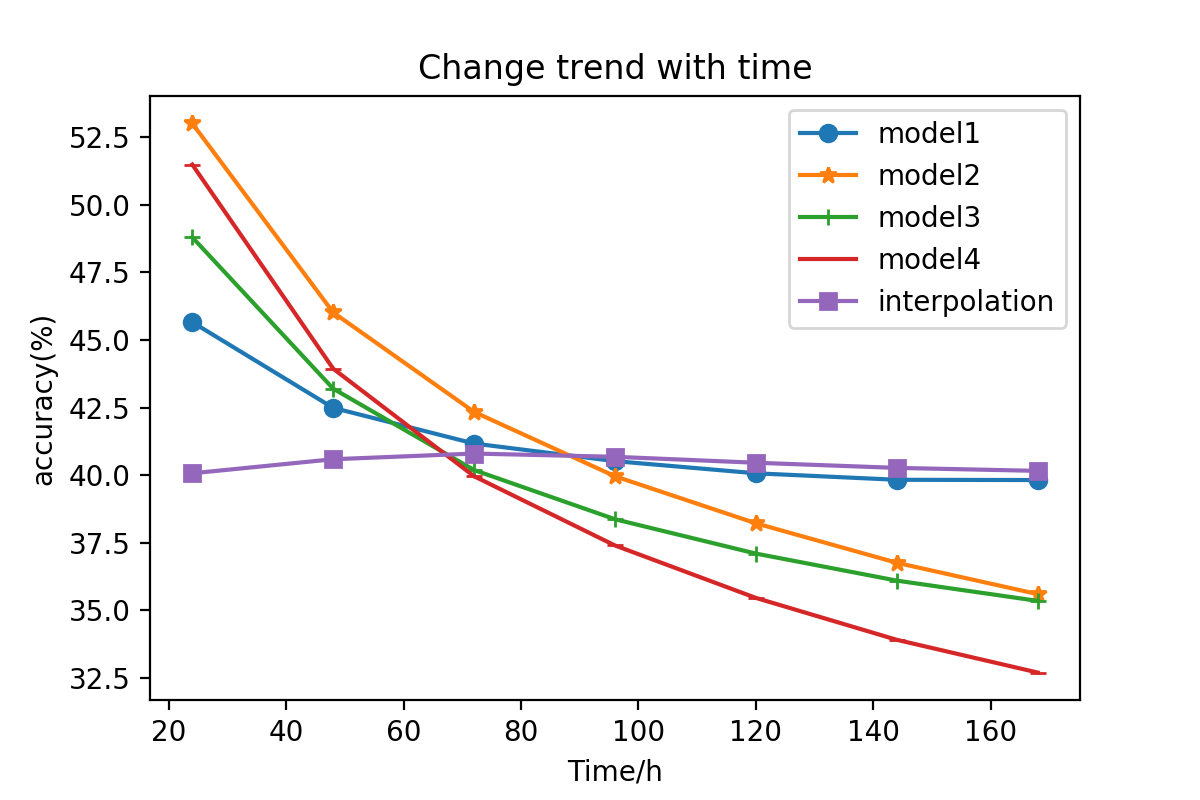
\includegraphics[width=0.45\textwidth]{accuracy.png}}}
\subfloat[均方误差变化]{\label{fig:rsmeacc}{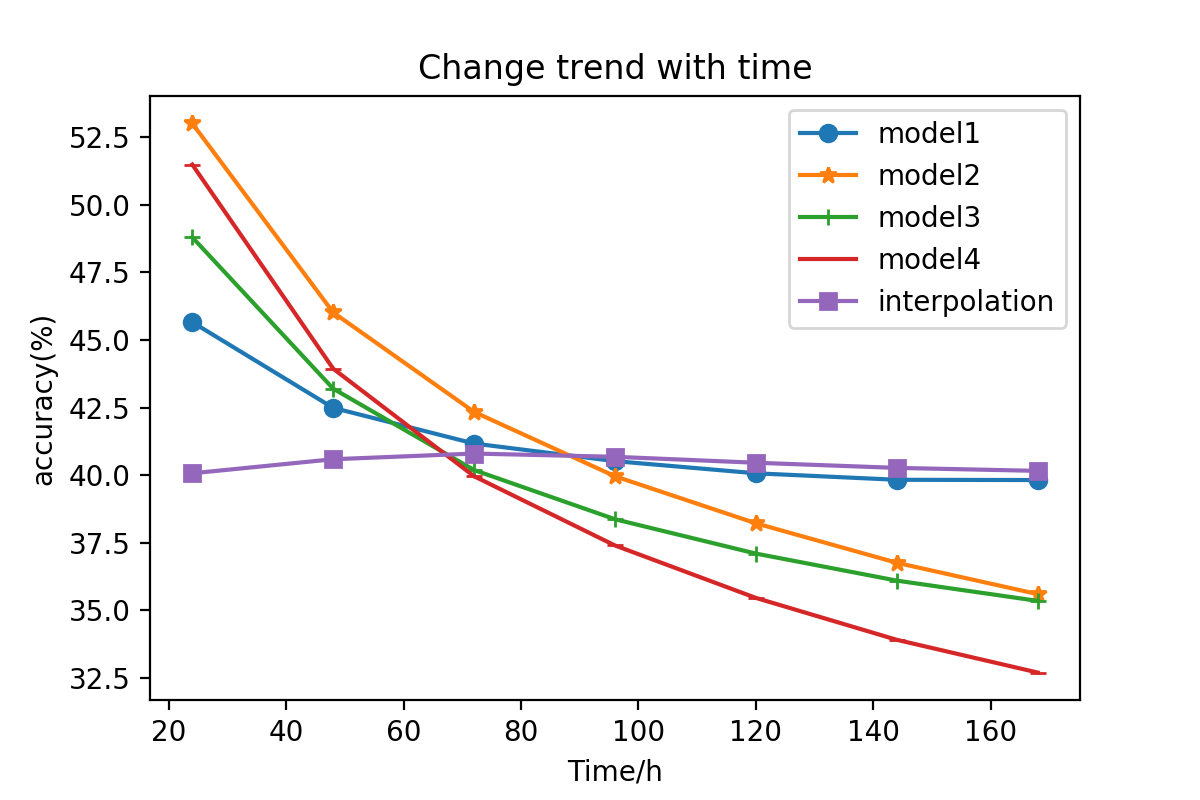
\includegraphics[width=0.45\textwidth]{accuracy.png}}}
\hfill
\caption{模型预测精度随着预测时间的变化}
%\label{fig:subfigures}
\end{figure}
加上RSME的误差分析部分
\subsection*{参数的影响}
上面的分析表明,所设计的残差网络在预测的精度上无论是简单的深度神经网络还是和均值比较都有较大的提升,而从表(\ref{table:diffpara})中也可以看出,采用不同的参数对于残差网络训练结果的影响:
\begin{itemize}
	\item 初始学习率
	\item 学习衰减指数
	\item 优化方法
\end{itemize}
\subsection{结果可视化和区域分析}
对于预测结果可以分别采用热力图和结合地理信息的人流地图加以可视化,如图(\ref{fig:peopleheatmap})所示:

\begin{figure}[ht]
\centering
\subfloat[人口热力图]{\label{fig:heatmap}{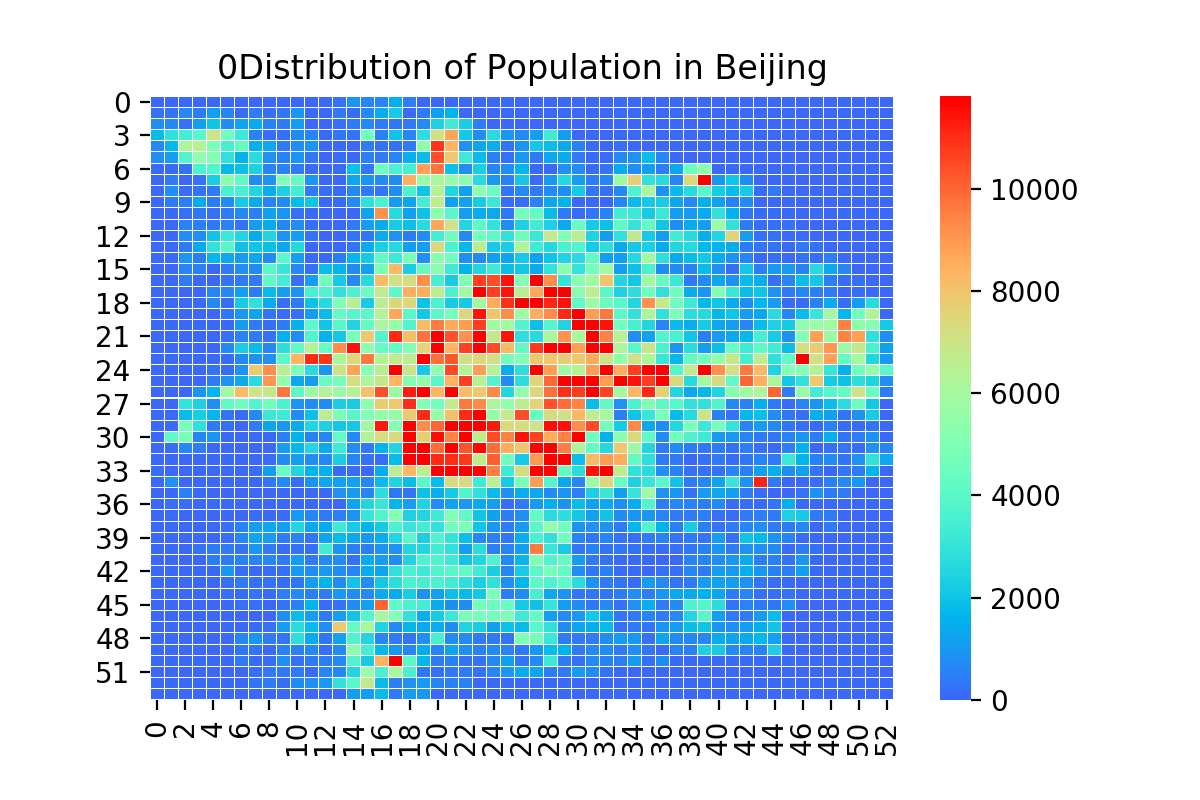
\includegraphics[width=0.45\textwidth]{heatmap.png}}}
\subfloat[结合实际地理信息的可视化]{\label{fig:folium}{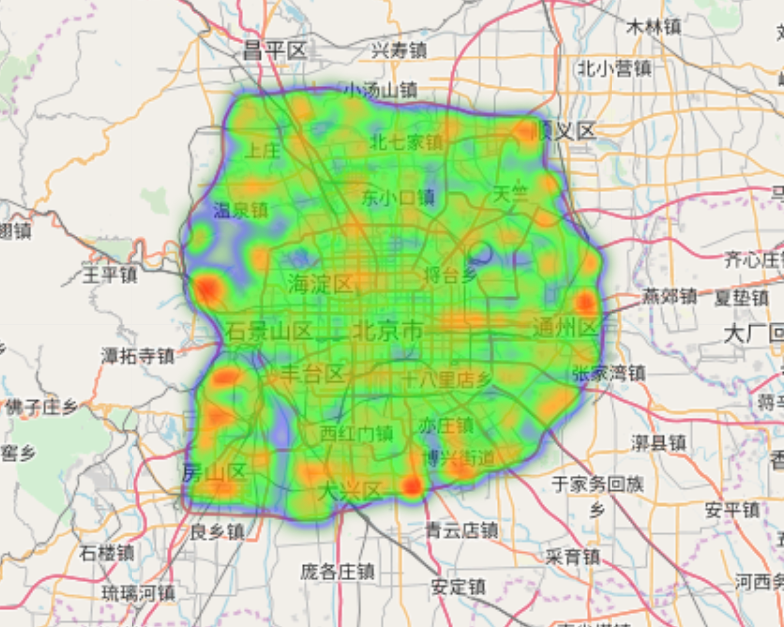
\includegraphics[width=0.45\textwidth]{folium.png}}}
\hfill
\caption{人口分布预测结果可视化}
\label{fig:peopleheatmap}
\end{figure}
而更进一步的,在对于全局预测效果的评估的基础上,可以更加细致的对于具体的特征地区进行预测结果的分析:
\begin{figure}[ht]
\centering
\subfloat[三里屯]{\label{fig:11}{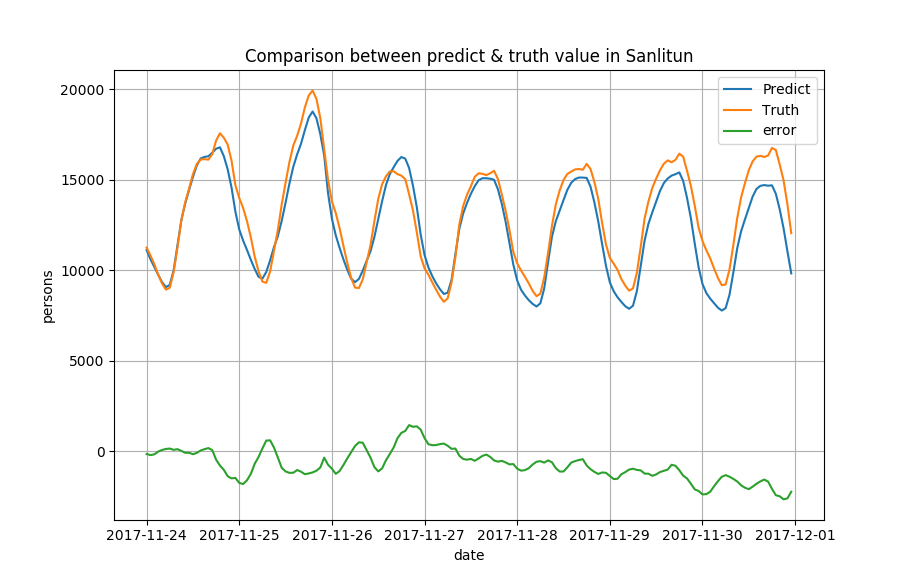
\includegraphics[width=0.45\textwidth]{region1.png}}}
\subfloat[天安门]{\label{fig:22}{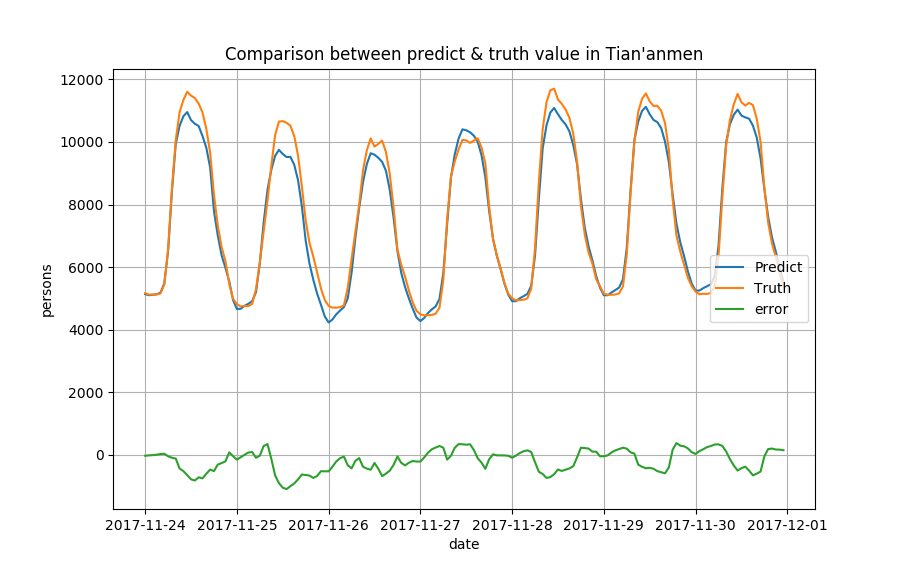
\includegraphics[width=0.45\textwidth]{region2.png}}}
\hfill
\subfloat[北京西站]{\label{fig:33}{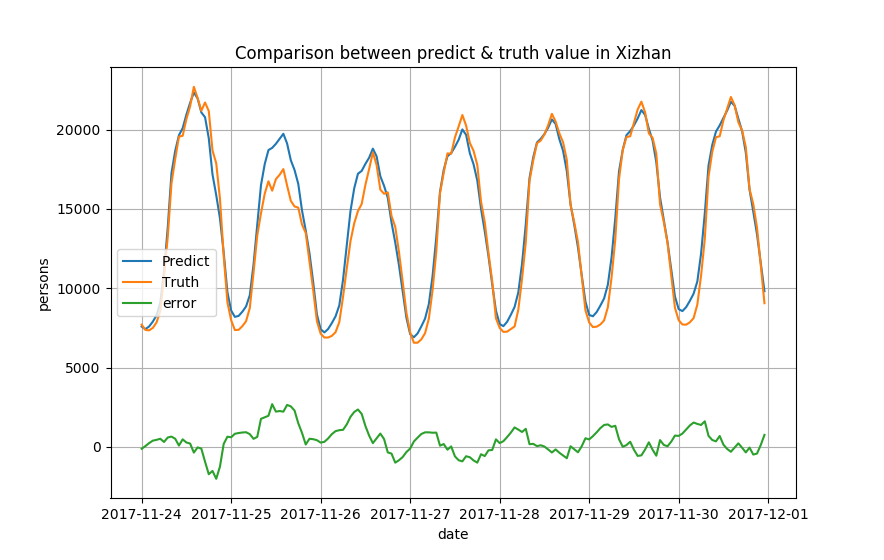
\includegraphics[width=0.45\textwidth]{region3.png}}}
\subfloat[中关村]{\label{fig:44}{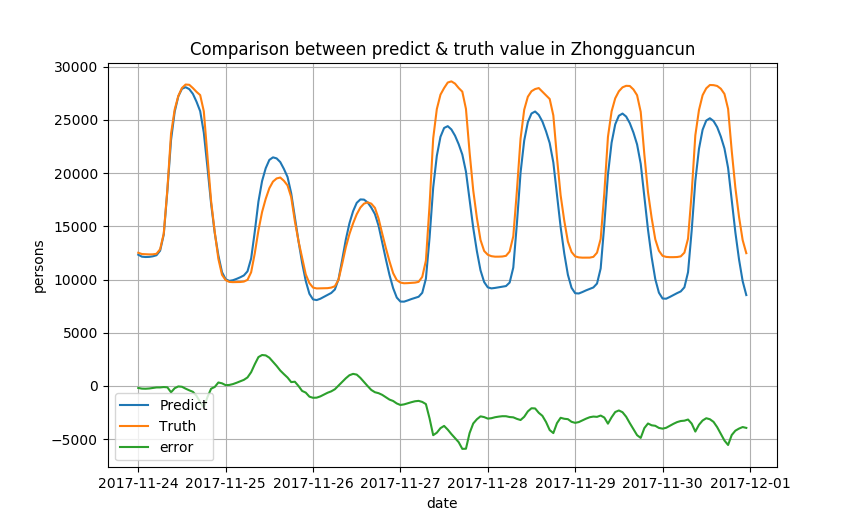
\includegraphics[width=0.45\textwidth]{region4.png}}}
\caption{四个典型地区的预测结果和真实值比较}
\label{fig:region}
\end{figure}
图(\ref{fig:11})展示了三里屯地区的人流量预测情况及其与真实值之间的对比关系,从曲线的走势可以看出,总体上预测值和真实值的符合度比较高,误差值在前期的分布没有明显的趋势性,表明造成预测误差的一个重要原因可能是随机因素的影响,而预测的后期也呈现出一定的预测精度的下降趋势,这也和之前的讨论分析是相符合的。\\
而图(\ref{fig:33})中展示了北京西站这样一个人流量较大但也有较明显变化的区域的预测结果,可以看出,对于高峰的预测是相对比较准确的,可以看出本模型可以在诸如火车站、地铁站等的人流预测和预警中发挥较好的作用。

\section{总结和展望}